\section{Combining Convolution and Recursive Neural Networks}\label{sec:cnn-treelstm}

Our model architecture is shown in Fig.~\ref{fig:cnntreelstm}.
The model has three modules: word embedding layer, convolution layer, and Constituency Tree-LSTM.

\begin{figure} [H]
    \centering
    \usetikzlibrary{matrix}
\usetikzlibrary{patterns}
\tikzset{
	sq1/.style={rectangle, minimum width=0.5cm, minimum height=0.5cm, text centered, draw=black},
	sq1m/.style={rectangle, minimum width=0.7cm, minimum height=0.3cm, text centered, draw=black},
	sq1p/.style={rectangle, minimum width=0.5cm, minimum height=0.5cm, text centered, draw=black, pattern=north west lines},
	circ/.style={circle, minimum width=0.3cm, minimum height=0.3cm, text centered, draw=black},
	arrow/.style={thick,->},
	sqvec/.style={matrix,matrix of nodes,nodes in empty cells},
}
\tikzstyle{cir} = [circle, minimum width=0.7cm, minimum height=0.7cm, text centered, draw=black ]

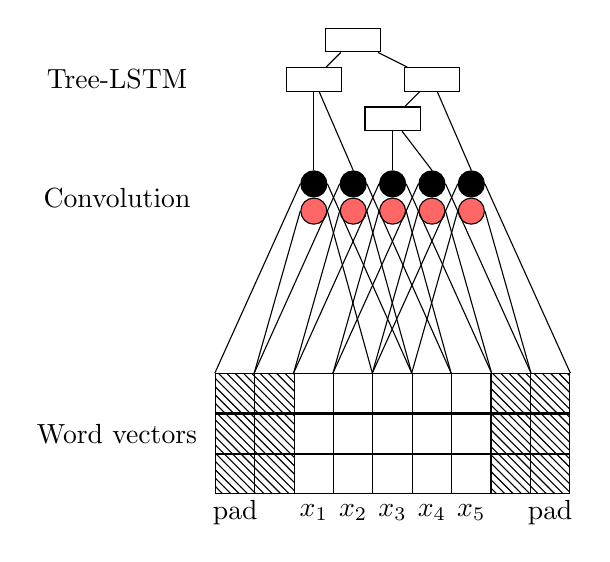
\begin{tikzpicture}
\node [sqvec,nodes={circ},      
every even row/.style = { nodes={fill=red!60}},
every odd row/.style = { nodes={fill=black!100}}] (c1) at (1.5,8.5) {
	\\
	\\ 
};  

\node [sqvec,nodes={circ},      
every even row/.style = { nodes={fill=red!60}},
every odd row/.style = { nodes={fill=black!100}}] (c2) at (2,8.5) {
	\\
	\\ 
};  

\node [sqvec,nodes={circ},      
every even row/.style = { nodes={fill=red!60}},
every odd row/.style = { nodes={fill=black!100}}] (c3) at (2.5,8.5) {
	\\
	\\ 
};  

\node [sqvec,nodes={circ},      
every even row/.style = { nodes={fill=red!60}},
every odd row/.style = { nodes={fill=black!100}}] (c4) at (3,8.5) {
	\\
	\\ 
};  

\node [sqvec,nodes={circ},      
every even row/.style = { nodes={fill=red!60}},
every odd row/.style = { nodes={fill=black!100}}] (c5) at (3.5,8.5) {
	\\
	\\ 
};  


\node [sqvec,column sep=-\pgflinewidth,nodes={sq1}] (v) at (2.5,5.5) {
	&&&&\\
	&&&&\\
	&&&&\\
};   

\node [sqvec,column sep=-\pgflinewidth,nodes={sq1p}] (v1) at (1,5.5) {
	\\
	\\
	\\
};   
\node [sqvec,column sep=-\pgflinewidth,nodes={sq1p}] (v2) at (0.5,5.5) {
	\\
	\\
	\\
};   
\node [sqvec,column sep=-\pgflinewidth,nodes={sq1p}] (v3) at (4,5.5) {
	\\
	\\
	\\
};   
\node [sqvec,column sep=-\pgflinewidth,nodes={sq1p}] (v4) at (4.5,5.5) {
	\\
	\\
	\\
};   

\draw (v1-1-1.north west) -- (c1-2-1.west); % inner left
\draw (v-1-3.north west) -- (c1-2-1.east); % inner right
\draw (v2-1-1.north west) -- (c1-1-1.west); % outer left
\draw (v-1-4.north west) -- (c1-1-1.east); % outer right

\draw (v-1-1.north west) -- (c2-2-1.west); % inner left
\draw (v-1-4.north west) -- (c2-2-1.east); % inner right
\draw (v1-1-1.north west) -- (c2-1-1.west); % outer left
\draw (v-1-5.north west) -- (c2-1-1.east); % outer right

\draw (v-1-2.north west) -- (c3-2-1.west); % inner left
\draw (v-1-5.north west) -- (c3-2-1.east); % inner right
\draw (v-1-1.north west) -- (c3-1-1.west); % outer left
\draw (v-1-5.north east) -- (c3-1-1.east); % outer right

\draw (v-1-3.north west) -- (c4-2-1.west); % inner left
\draw (v-1-5.north east) -- (c4-2-1.east); % inner right
\draw (v-1-2.north west) -- (c4-1-1.west); % outer left
\draw (v3-1-1.north east) -- (c4-1-1.east); % outer right

\draw (v-1-4.north west) -- (c5-2-1.west); % inner left
\draw (v3-1-1.north east) -- (c5-2-1.east); % inner right
\draw (v-1-3.north west) -- (c5-1-1.west); % outer left
\draw (v4-1-1.north east) -- (c5-1-1.east); % outer right


\node [sq1m] (v8) at (2,10.5) {};
\node [sq1m] (v7) at (1.5,10) {};
\node [sq1m] (v6) at (3,10) {};
\node [sq1m] (v5) at (2.5,9.5) {};
% \draw  (c3) edge (v5);
% \draw  (c4) edge (v5);
\draw  (v5) edge (v6);
% \draw  (c5) edge (v6);
% \draw  (c1) edge (v7);
\draw  (v7) edge (v8);
% \draw  (c2) edge (v7);
\draw  (v6) edge (v8);



\node at (0.5,4.5) {pad};
% \node at (1,4) {pad};
\node at (1.5,4.5) {$x_1$};
\node at (2,4.5) {$x_2$};
\node at (2.5,4.5) {$x_3$};
\node at (3,4.5) {$x_4$};
\node at (3.5,4.5) {$x_5$};
\node at (4.5,4.5) {pad};
% \node at (4.5,4) {pad};

\node at (-1,8.5) {Convolution};
\node at (-1,5.5) {Word vectors};
\node at (-1,10) {Tree-LSTM};

% connect lstm to circle
\draw  (v7) edge (c1-1-1.north);
\draw  (v7) edge (c2-1-1.north);
\draw  (v5) edge (c3-1-1.north);
\draw  (v5) edge (c4-1-1.north);
\draw  (v6) edge (c5-1-1.north);
\end{tikzpicture}
    \caption[CNN-Tree-LSTM]{CNN-Tree-LSTM}
    \label{fig:cnntreelstm} % label MUST come after caption
\end{figure}

\subsection{Word Embedding Layer}
Suppose that \(Z = \{e_0, e_1, \ldots e_m\}\) is a set input channels with each channel uses a different word embedding.
The first word in a sentence is indexed as word-\(0\)th.
If the sentence is padded with dummy words, left padded dummy words are indexed by negative integers.

For any word embedding~\(e\), the vector presentation of the word-\(i\)th is denoted as~\(w^{(e)}_i \in \mathbb{R}^{d_e}\).
The vector presentation of word-\(i\)th through the set of input channels \(Z\) is expressed as follow:
\begin{align}
 x_i &= w^{(e_0)}_i \ominus w^{(e_1)}_i \ominus  \ldots \ominus w^{(e_m)}_i&\label{concat-emb}
\end{align}
In Eq.\eqref{concat-emb}, \(\ominus\) is concatenation operator which results in the vector \(x_i \in \mathbb{R}^{d}\) with \(d = \sum_{e \in Z} d_e\).
Any sequence of words starting from word-\(i\)th to word-\(j\)th is present as the following matrix:
\begin{align}
X_{i:j} &= x_i \oplus x_{i+1} \oplus \ldots \oplus x_j &\label{concat}
\end{align}
In Eq.\eqref{concat}, \(\oplus\) is concatenation operator which results in the matrix \(X_{i:j} \in \mathbb{R}^{d \times (j-i+1)}\).
\subsection{Convolution Layer}\label{sec:cnn}
Given that \(F\) is the set of all filters of the convolution layer, for any filter \(v \in F\) which has window size \(l\) and set of parameters \(\theta^{(v)} = \{ W^{(v)}, b^{(v)} | W^{(v)} \in \mathbb{R}^{d \times l}, b^{(v)} \in \mathbb{R}\}\), filter \({v}\) is applied on any sequence of word-\(i\)th to word-\((i+l-1)\)th through the following equation:
\begin{align}
c^{(v)}_j &= f(W^{(v)} \otimes X_{i:i+l-1} + b^{(v)}) &\label{filter}
\end{align}
In Eq.\eqref{filter}, operator \(\otimes\) is the Hadamard product~\cite{element-prod}.
\(b \in \mathbb{R}\) is bias term. \(f\) is an activation function.
For indexing, \(j = i + x\) with \(x \in \mathbb{N}\) and \(0 \leq x < l\).
If half-padding policy is employed then \(j = i + \floor{\frac{l}{2}}\).

By slicing the filter \(v\) through the sentence (i.e. applying the filter \(v\) on different sequences of length \(l\) along the sentence) we get vector \(c^{(v)} = [c^{(v)}_0, c^{(v)}_1~\cdots]\) which is a feature map of the sentence~\(s\).
The length of the feature map \(c^{(v)}\) depends on the length of the input sentence, the way which filter \(v\) was slided through the sentence and its window size \(l\)~\cite{conv-arith}.

In our model, all filters in \(F\) are restricted to have odd window sizes and being applied on the sentence according to half padding, unit strides policy~\cite{conv-arith}.
These conditions guarantee that the lengths of all feature maps produced from a sentence are equal to the number of words in that sentence~\cite{conv-arith}.

Suppose the size of the set of filters \(F\) is \(m\), all the feature maps of a sentence of length \(n\) produced by the set of filters is concatenated into one matrix \(P \in \mathbb{R}^{m \times n}\).
The \(i\)-th column vector of \(P\) are treated as the vector representation of the \(i\)-th word in the sentence.


\subsection{Recurrent Neural Network}
\subsubsection{Vanilla Recurrent unit}\label{sec:vanilla-rnn}
Denoting input sequence as \(I = \{i_0,\ldots,i_n\}, \forall t, i_t \in \mathbb{R}^n\), Vanilla Recurrent unit is expressed as the following recursive formula~\cite{treeLSTM}:
\begin{align}
h_t &= tanh(Wi_t + Uh_{t-1} + b)&
\end{align}
For sentence-level sentiment analysis, \(h_n\) is treated as output of the network.
In theory, Vanilla Recurrent Neural Network is Turing-Complete~\cite{rnn-turing-complete} but difficult to train, especially on long input sequence, due to the problems of exploding and vanishing gradient~\cite{Bengio1994}.
Long Short Term Memory unit (LSTM)~\cite{originLSTM} unit was invented to mitigate the problem of vanishing gradient.
\subsubsection{Long Short Term Memory unit}\label{sec:lstm}
Long Short Term Memory unit ~\cite{originLSTM} is expressed as the following recursive formula:
\begin{align}
w_t &= \sigma\left(W^{(w)}i_t + U^{(w)}h_{t-1} + b^{(w)}\right) \label{eq:lstm-input-gate}&\\
f_t &= \sigma\left(W^{(f)}i_t + U^{(f)}h_{t-1} + b^{(f)}\right) \label{eq:lstm-forget-gate}&\\
o_t &= \sigma\left(W^{(o)}i_t + U^{(o)}h_{t-1} + b^{(o)}\right) \label{eq:lstm-output-gate}&\\
u_t &= tanh\left(W^{(u)}i_t + U^{(u)}h_{t-1} + b^{(u)}\right) \label{eq:lstm-update-gate}&\\
c_t &= r_t \odot u_t + f_t \odot c_{t-1} \label{eq:longterm-mem}&\\
h_t &= o_t \odot tanh(c_t) \label{eq:temperal-mem}&
\end{align}
The operation \(\odot\) denotes the element-wise vector product.
Traditionally, \(w_t\), \(f_t\) and \(o_t\) are called input/write gate, forget/deallocate gate and output/read gate respectively and \(c_t\) is called memory cell.
% MAY NOT NECCESSARY
Intuitively, we can interpret how the network works as follow:
\begin{itemize}
  \item \(h_{t-1}\) can be viewed as a short-term memory of the network
  \item \(u_t\) is the information extracted from in current input \(i_t\) and the short-term memory \(h_{t-1}\)
  \item Write gate \(w_t\) decides which information from \(u_t\) will be written into the memory cell \(c_t\)
  \item Forget gate \(f_t\) decides which information will be preserved on memory cell \(c_t\)
  \item \(o_t\) decides which information will be read from the memory cell \(c_t\), which will produce the short-term memory \(h_t\).
\end{itemize}

% in the above formula, \(h_{t-1}\) can be viewed as a short-term memory of the network;
% \(u_t\) is the information extracted from in current input \(i_t\) and the short-term memory \(h_{t-1}\);
% write gate \(w_t\) decides which information from \(u_t\) will be written into the memory cell \(c_t\);
% forget gate \(f_t\) decides which information will be preserved on memory cell \(c_t\);
% and \(o_t\) decides which information will be read from the memory cell \(c_t\), which will produce the short-term memory (or output) \(h_t\).


\subsection{Constituency Tree-LSTM}\label{treelstm}
Let \(d\) be the size of the input vectors, \(r
\) be the size of the memory cell and \(z\) be the number of sentiment classes.
\paragraph{Leaf module}
Given any input vector \(x \in \mathbb{R}^d\), the calculation steps inside the leaf module is expressed as follow:
\begin{align}
o &= \sigma{\left( W^{(o)} x + a^{\left(o\right)}\right)} & \\
c &= W^{(c)} x + a^{(c)} & \\
h &= o \odot \tanh{\left(c\right)} &
\end{align}
In this module, \(W^{(o)}, W^{(c)} \in \mathbb{R}^{r \times d}\) and \(a^{\left(o\right)}, a^{(c)} \in \mathbb{R}^r\).
\paragraph{Composer module}
Given the input vectors \({h_l}\) and \({c_l}\) from the left child node, \({h_r}\) and \({c_r}\) from the right child node, the calculation steps inside the composer module are expressed as follow:
\begin{align}
i &= \sigma{ \left(U_l^{(i)} h_{l} + U_r^{(i)} h_{r} + b^{(i)} \right) } &\\
f_{l} &= \sigma{\left(U_{l}^{(l)} h_{l} + U_{r}^{(l)} h_{r} + b^{(f)}\right)} & \\
f_{r} &= \sigma{\left(U_{l}^{(r)} h_{l} + U_{r}^{(r)} h_{r} + b^{(f)}\right)} & \\
o &= \sigma{\left( U_l^{(o)} h_{l} + U_r^{(o)} h_{r} + b^{(o)}\right)} &\\
u &= \tanh{\left( U_l^{(u)} h_{l} + U_r^{(u)} h_{r} + b^{(u)}\right)} &\\
c &= i \odot u + f_{l} \odot c_{l} + f_{r} \odot c_{r} & \\
h &= o \odot \tanh{\left(c\right)} &
\end{align}
For any \(j \in \{i, l, r, o, u\}\) and \(x \in \{l, r\}\), \(U_x^{(j)} \in \mathbb{R}^{r \times r}\) and \( b^{(j)} \in \mathbb{R}^r\).

\paragraph{Output module}
Denoting sequence of words spanned by a sub-tree rooted at node \({j}\) as \({\{x\}_j}\).
Given \({h_j}\) of node \({j}\), the prediction at node \({j}\) is computed by the output module as follow:
\begin{align}
\hat{p_{\theta}}(y \mid \{x\}_j ) &= softmax( W^{(s)} h_j + b^{(s)}) & \\
\hat{y_j} &= \underset{y}{\mathrm{argmax}} \; \hat{p_{\theta}}(y \mid \{x\}_j ) &
\end{align}
With \(W^{(s)} \in \mathbb{R}^{z \times r}\) and \( b^{(s)} \in \mathbb{R}^z\).
\paragraph{Composing sentence}
% Given any sentence, its parse tree and set of vectors representation of each word in the sentence, Constituency Tree-LSTM is applied on the sentence as follow:
% For any non-leaf node, composer module is applied recursively and for any leaf node, the leaf module is applied on the vector representation of the corresponding word.
% Finally, we can apply the output module on any node in the parse tree.
Given any sentence, its parse tree and set of vectors representation of each word in the sentence, Constituency Tree-LSTM is applied on the sentence as follow:
\begin{itemize}
  \item At leaf node, leaf module takes input from previous layer (convolution layer) output of corresponding word.
  \item At non-leaf node, composer module is applied recursively.
  \item In addition, at every node \({j}\), output module takes input from leaf module or composer module to predict sentiment of sub-tree root \({j}\).
\end{itemize}

